% fig_5_1_methodology_pipeline.tex
% Standalone TikZ diagram: Methodology pipeline for text classification thesis
\documentclass[tikz,border=5pt]{standalone}

\usepackage[T1]{fontenc}
\usepackage{amsmath,amssymb}

\usetikzlibrary{shapes, arrows.meta, positioning, fit, calc, decorations.pathmorphing}

% ── Colour palette (pastel / academic) ──────────────────────────────────────
\definecolor{colData}{RGB}{186,215,242}       % light blue
\definecolor{colLLM}{RGB}{186,237,193}        % light green
\definecolor{colEnc}{RGB}{211,196,232}        % light purple
\definecolor{colFilt}{RGB}{253,213,170}       % light orange
\definecolor{colWeight}{RGB}{255,245,186}     % light yellow
\definecolor{colClf}{RGB}{245,195,210}        % light pink
\definecolor{colAccept}{RGB}{56,142,60}       % green (accepted)
\definecolor{colReject}{RGB}{198,40,40}       % red   (rejected)
\definecolor{colResult}{RGB}{33,33,33}        % dark grey for result box

% ── Reusable node styles ────────────────────────────────────────────────────
\tikzset{
  % shared base
  stage/.style={
    rectangle, rounded corners=6pt,
    draw=#1!70!black, line width=0.8pt,
    fill=#1, fill opacity=0.85, text opacity=1,
    inner sep=8pt, outer sep=2pt,
    font=\small, align=center,
    minimum height=2.4cm, minimum width=3.1cm,
  },
  % per-stage shortcuts
  sData/.style   ={stage=colData},
  sLLM/.style    ={stage=colLLM},
  sEnc/.style    ={stage=colEnc},
  sFilt/.style   ={stage=colFilt, line width=1.4pt,
                    minimum height=4.6cm, minimum width=3.6cm},
  sWeight/.style ={stage=colWeight},
  sClf/.style    ={stage=colClf, minimum width=3.4cm},
  % arrows
  mainArr/.style ={-Stealth, thick, draw=black!70},
  labelArr/.style={font=\scriptsize, text=black!70, midway},
}

\begin{document}
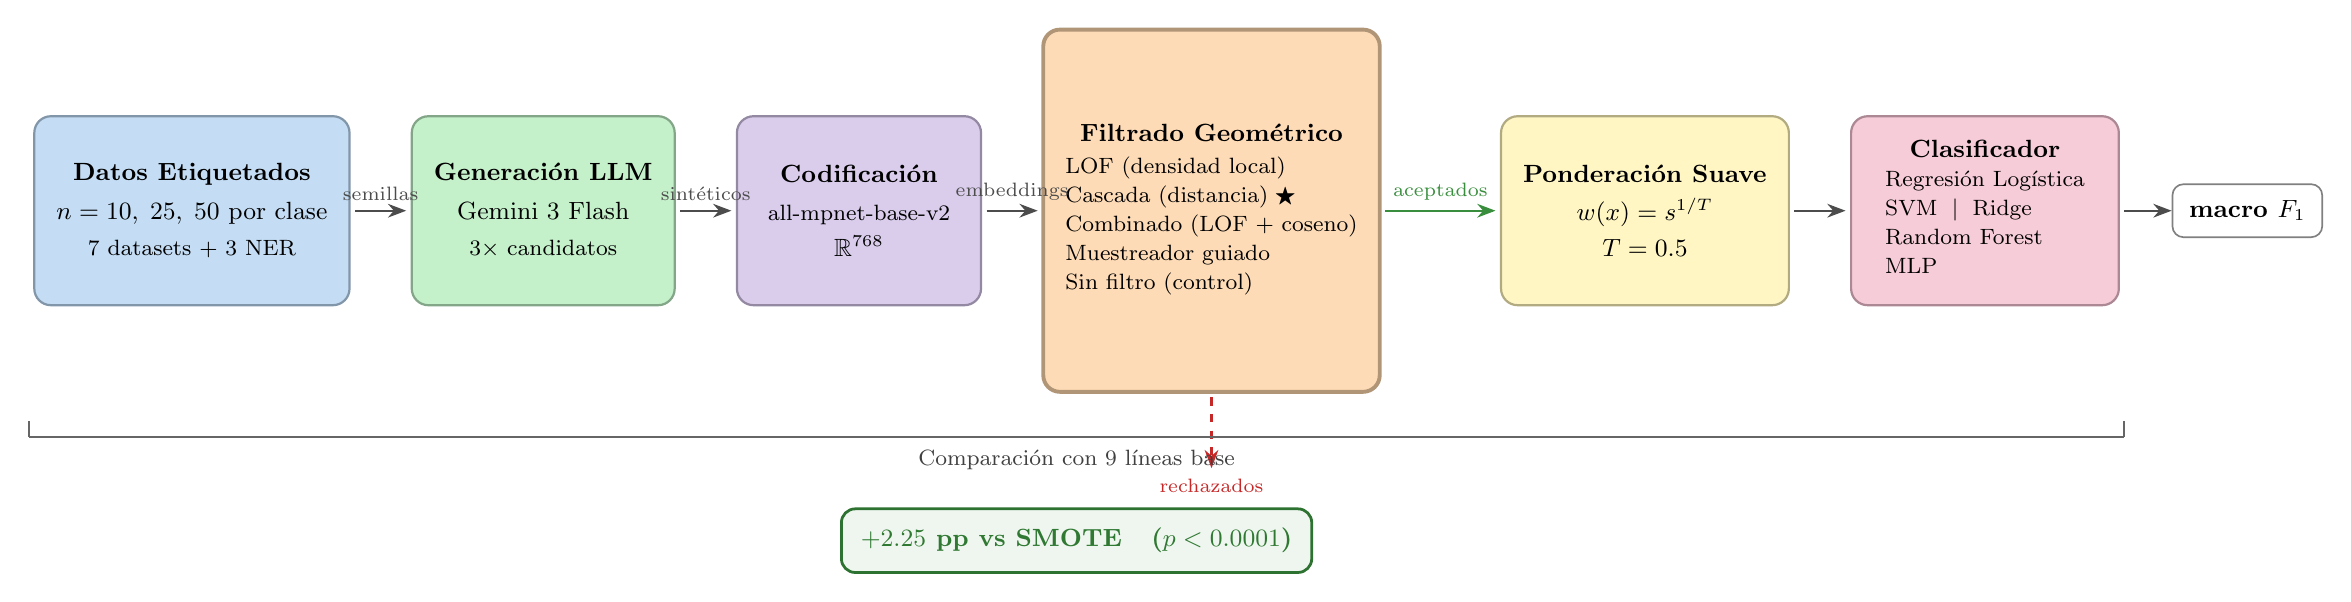
\begin{tikzpicture}[node distance=1.1cm and 0.65cm]

% ═══════════════════════════════════════════════════════════════════════════
%  STAGE 1 – Datos Etiquetados
% ═══════════════════════════════════════════════════════════════════════════
\node[sData] (data) {%
  \textbf{Datos Etiquetados}\\[3pt]
  $n = 10,\;25,\;50$ por clase\\[2pt]
  {\footnotesize 7 datasets $+$ 3 NER}%
};

% ═══════════════════════════════════════════════════════════════════════════
%  STAGE 2 – Generaci\'{o}n LLM
% ═══════════════════════════════════════════════════════════════════════════
\node[sLLM, right=of data] (llm) {%
  \textbf{Generaci\'{o}n LLM}\\[3pt]
  Gemini 3 Flash\\[2pt]
  {\footnotesize $3\times$ candidatos}%
};

% ═══════════════════════════════════════════════════════════════════════════
%  STAGE 3 – Codificaci\'{o}n
% ═══════════════════════════════════════════════════════════════════════════
\node[sEnc, right=of llm] (enc) {%
  \textbf{Codificaci\'{o}n}\\[3pt]
  {\footnotesize all-mpnet-base-v2}\\[2pt]
  $\mathbb{R}^{768}$%
};

% ═══════════════════════════════════════════════════════════════════════════
%  STAGE 4 – Filtrado Geom\'{e}trico  (core block)
% ═══════════════════════════════════════════════════════════════════════════
\node[sFilt, right=of enc] (filt) {%
  \textbf{Filtrado Geom\'{e}trico}\\[4pt]
  {\footnotesize
    \begin{tabular}{@{}l@{}}
      LOF (densidad local)\\[1pt]
      Cascada (distancia)\;$\bigstar$\\[1pt]
      Combinado (LOF $+$ coseno)\\[1pt]
      Muestreador guiado\\[1pt]
      Sin filtro (control)
    \end{tabular}%
  }%
};

% ═══════════════════════════════════════════════════════════════════════════
%  STAGE 5 – Ponderaci\'{o}n Suave
% ═══════════════════════════════════════════════════════════════════════════
\node[sWeight, right=1.4cm of filt] (weight) {%
  \textbf{Ponderaci\'{o}n Suave}\\[3pt]
  $w(x) = s^{1/T}$\\[2pt]
  $T = 0.5$%
};

% ═══════════════════════════════════════════════════════════════════════════
%  STAGE 6 – Clasificador
% ═══════════════════════════════════════════════════════════════════════════
\node[sClf, right=of weight] (clf) {%
  \textbf{Clasificador}\\[3pt]
  {\footnotesize
    \begin{tabular}{@{}l@{}}
      Regresi\'{o}n Log\'{i}stica\\[1pt]
      SVM \;\textbar\; Ridge\\[1pt]
      Random Forest\\[1pt]
      MLP
    \end{tabular}%
  }%
};

% ═══════════════════════════════════════════════════════════════════════════
%  MAIN CONNECTING ARROWS
% ═══════════════════════════════════════════════════════════════════════════
\draw[mainArr] (data)   -- node[labelArr, above] {semillas}    (llm);
\draw[mainArr] (llm)    -- node[labelArr, above] {sint\'{e}ticos} (enc);
\draw[mainArr] (enc)    -- node[labelArr, above] {embeddings}  (filt);

% accepted arrow (green, to the right)
\draw[mainArr, draw=colAccept, thick]
  (filt.east) -- node[labelArr, above, text=colAccept] {aceptados} (weight.west);

% rejected arrow (red, dashed, downward)
\draw[-Stealth, thick, dashed, draw=colReject]
  (filt.south) -- ++(0,-0.9)
  node[below, font=\scriptsize, text=colReject] {rechazados};

\draw[mainArr] (weight) -- node[labelArr, above] {} (clf);

% ── Output: macro F1 ───────────────────────────────────────────────────────
\node[right=0.6cm of clf, font=\small\bfseries, align=center,
      draw=black!50, rounded corners=4pt, inner sep=6pt,
      fill=white, line width=0.6pt]
  (output) {macro $F_1$};
\draw[mainArr] (clf) -- (output);

% ═══════════════════════════════════════════════════════════════════════════
%  BOTTOM BRACKET – Comparison with baselines
% ═══════════════════════════════════════════════════════════════════════════
% horizontal span: from data.west to clf.east
\coordinate (bracL) at ($(data.south west) + (0,-1.6)$);
\coordinate (bracR) at ($(clf.south east)  + (0,-1.6)$);

% draw a brace-like shape with a simple line + ticks
\draw[thick, black!60]
  (bracL) -- (bracR)
  (bracL) -- ++(0,0.2)
  (bracR) -- ++(0,0.2);
% centre label
\node[below=0.05cm of {$(bracL)!0.5!(bracR)$},
      font=\footnotesize, text=black!75, align=center]
  (baseline) {Comparaci\'{o}n con 9 l\'{i}neas base};

% ═══════════════════════════════════════════════════════════════════════════
%  RESULT CALLOUT
% ═══════════════════════════════════════════════════════════════════════════
\node[below=0.35cm of baseline,
      rectangle, rounded corners=5pt,
      draw=colAccept!80!black, line width=1pt,
      fill=colAccept!8, inner sep=7pt,
      font=\small\bfseries, text=colAccept!85!black, align=center]
  (result) {$+2.25$ pp vs SMOTE\quad($p < 0.0001$)};

\end{tikzpicture}
\end{document}
